\documentclass{resume} % Use the custom resume.cls style

\usepackage[left=0.4 in,top=0.4 in,right=0.4 in,bottom=0.4 in]{geometry} % Document margins
\usepackage{graphicx} 
\newcommand{\tab}[1]{\hspace{.2667\textwidth}\rlap{#1}} 
\newcommand{\itab}[1]{\hspace{0em}\rlap{#1}} 
\name{ABHIK L SALIAN} % Your name
\address{+91 7411328238 \\ Mangaluru, Karnataka \\ \href{https://abhiksalian.github.io/portfolio/}{\textcolor{black}{abhiksalian.github.io/portfolio}}}
\address{\href{mailto:abhiksalian0728@gmail.com}{\textcolor{black}{abhiksalian0728@gmail.com}} \\ \href{https://linkedin.com/in/abhik-salian}{\textcolor{black}{linkedin.com/in/abhik-salian}} \\ \href{https://www.github.com/AbhikSalian}{\textcolor{black}{github.com/AbhikSalian}}}

\begin{document}

% Top part with photo and details
% \begin{minipage}[t]{0.75\textwidth}
%     \vspace{-0.6in}
%     \LARGE \textbf{ABHIK L SALIAN} 
%     \vspace{0.3cm}
%     \\
%     \normalsize
%     +91 7411328238 \textbar{} 
%     Mangaluru, Karnataka \textbar{}
%     \href{https://abhiksalian.github.io/portfolio/}{\textcolor{black}{abhiksalian.github.io/portfolio}} 
%     \vspace{0.15cm}
%     \\
%     \href{mailto:abhiksalian0728@gmail.com}{\textcolor{black}{abhiksalian0728@gmail.com}} \textbar{}
%     \href{https://linkedin.com/in/abhik-salian}{\textcolor{black}{linkedin.com/in/abhik-salian}} \textbar{}
%     \href{https://www.github.com/AbhikSalian}{\textcolor{black}{github.com/AbhikSalian}}
% \end{minipage}
% \begin{minipage}[t]{0.25\textwidth}
%     \vspace{-0.8in}
%     \begin{flushright}
%         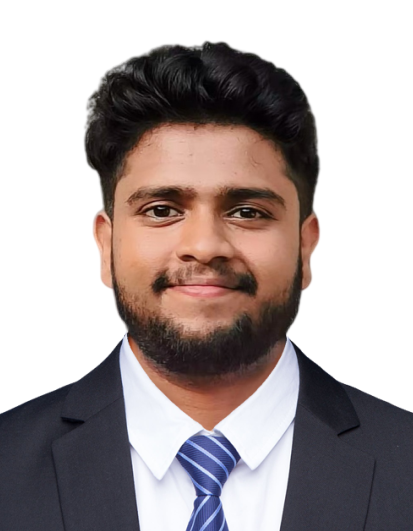
\includegraphics[width=0.85in]{Abhik_L_Salian.png} % Replace with your photo filename
%     \end{flushright}
% \end{minipage}


%----------------------------------------------------------------------------------------
%	OBJECTIVE
%----------------------------------------------------------------------------------------

\begin{rSection}{PROFILE}
{
    As a dedicated Computer Science undergraduate 
    % and an unlicensed UAV pilot 
    with a consistent 
    academic record, I am always eager to expand my knowledge 
    and skills. With a solid foundation in core Computer Science
    % and software development 
    principles, I am looking forward to start my career and 
     apply what I've learned to real-world projects.
}
% {As a Computer Science undergraduate with a consistent academic record,
%  I am eager to learn new things every day. 
%  I have a solid grasp of key fundamentals of Computer Science topics and 
%  am excited to begin my career by applying my knowledge and skills to 
%  real-world projects.
% }
% {
%     Computer Science undergraduate, an aviation enthusiast and an unlicensed UAV pilot, eager to kickstart my
% career and contribute to innovative projects. Good grip on topics related to aviation, proficient in algorithms,
% data structures, and software development principles, ready to tackle real-world challenges.
% }

\end{rSection}
%----------------------------------------------------------------------------------------
%	EDUCATION SECTION
%----------------------------------------------------------------------------------------

\begin{rSection}{Education}

{\bf Bachelor of Engineering} \textbar{} St. Joseph Engineering College, Mangaluru \hfill {2021 - present}\\
Computer Science and Engineering \textbar{} CGPA - 9.47/10

{\bf Higher Secondary} \textbar{} St. Aloysius PU College, Mangaluru \hfill {2019 - 2021}\\
PCME \textbar{} Percentage - 98\%

% {\bf High School}, St. Aloysius High School, Urwa, Mangaluru \hfill {2009 - 2019}\\
% SSLC \textbar{} Percentage - 95.52\%
%Minor in Linguistics \smallskip \\
%Member of Eta Kappa Nu \\
%Member of Upsilon Pi Epsilon \\


\end{rSection}

%----------------------------------------------------------------------------------------
% TECHINICAL STRENGTHS	
%----------------------------------------------------------------------------------------
\begin{rSection}{SKILLS}

\begin{tabular}{ @{} >{\bfseries}l @{\hspace{6ex}} l }
Technical Skills & C, Java, Python, 
Git, 
HTML, CSS, JavaScript, React,
  Node,
MySQL, PHP,
MongoDB
%    WordPress,
    % SolidWorks
% Technical Skills & C, Java, Python, SolidWorks, Ansys, HTML, CSS, JavaScript, MySQL, Matlab, PHP
\\
Soft Skills & Adaptability, Interpersonal Communication, Leadership, Punctual, Time Management\\
% Other Skills & UAV Piloting, RC Aircraft and Drone Fabrication\\
\end{tabular}
\end{rSection} 

\begin{rSection}{INTERNSHIPS}

\textbf{Salesforce Administrator Virtual Internship} \hfill Oct 2023 - Nov 2023\\
Certified by SmartInternz \hfill \textit{Virtual Internship}
 \begin{itemize}
    \itemsep -3pt {} 
    \item This internship helped me gain hands-on experience in managing and configuring the Salesforce platform.
    \end{itemize}
 
 \textbf{Web Developer Intern} \hfill Oct 2023 - Nov 2023\\
Glowtouch Technologies Pvt. Ltd. \hfill \textit{Mangaluru, Karnataka}
 \begin{itemize}
    \itemsep -3pt {} 
    %  \item Carried out 4-week internship in the web development domain.
    %  \item Worked on full-stack web projects under the guidance of industry mentors.
    \item Developed a full-stack web app `SmartStitch', designed for the clients of tailors to ease their tailoring process. 
 \end{itemize}

\end{rSection} 


%----------------------------------------------------------------------------------------
% CERTIFICATIONS
%------------------------------------------------------------------------------------------
\begin{rSection}{Certifications} 
    %     \textbf{Salesforce Administrator} \hfill Nov 2023\\
    % Certified by SmartInternz %\hfill \textit{Mangaluru, Karnataka}
    %  \begin{itemize}
    %     \itemsep -3pt {} 
    %     \item Through the certification, I learned to create and customize reports and dashboards for data analysis and business insights. 
    %      \item Developed problem-solving skills to address and resolve common issues within the Salesforce platform.
    %  \end{itemize}
        \begin{itemize}


            \item \textbf{TechA Blockchain Developer Certification} \hfill July 2024\\
            Certified in TechA Blockchain Development from Infosys Springboard, demonstrating proficiency in blockchain technologies, smart contract development, and Hyperledger Fabric administration.    
           
            \item \textbf{Google UX Design Certification} \hfill June 2024\\
            Certified UX Designer with a Google UX Design Professional Certificate and hands-on experience in user research, wireframing, prototyping, and usability testing. 
            % Adept at creating user-centered designs using tools like Figma and Adobe XD. Seeking to contribute to a dynamic team and create impactful user experiences.    


            % \item \textbf{Salesforce Administrator} \hfill Nov 2023\\
            % This certification helped me learn to create and customize reports and dashboards for data analysis and business insights.
            % Salesforce Administrator Certification validates skills in managing and configuring Salesforce.\\
            %    \\ Skills earned: Data management, Security, Industry awareness
   
            % \item \textbf{Information Technology - Concepts and Applications} \hfill May 2017\\
            % Completed two weeks of training on basics of Computer Science concepts under \textbf{Spark: Catch Them Young} programme conducted by \textbf{Infosys Limited, Mangalore} Development Centre.

        \end{itemize}
        
        
        \end{rSection}
         

%----------------------------------------------------------------------------------------
%	WORK EXPERIENCE SECTION
%----------------------------------------------------------------------------------------

\begin{rSection}{PROJECTS}
\begin{itemize}

    \item \textbf{B-LOCK: A Blockchain based e-vault application}{, is 
    an application designed using React JS to securely store and manage 
    files using Blockchain Technology. 
    % Utilizing the Ethereum blockchain, B-LOCK ensures file integrity, security, and transparency.
    }

% \item Worked as a freelancer on \textbf{WordPress site} built using \textbf{Elementor} for a UAE-based company that delivers POS solutions. I contributed towards the implementation of \textbf{ContactForm7} plugin integration.

\item \textbf{SmartStitch: A smart application for your tailoring needs}{, is an innovative web platform designed to streamline the process of ordering tailor-made dresses. 
% Clients can easily provide their measurements and place orders without the need to visit a tailor in person.
}
% \item \textbf{Impact test on RC Aircraft using Ansys}{, Conducted research and wrote a paper on the impact that a radio-controlled aircraft sustains during various scenarios such as hard belly landing and nose landing.}

% \textbf{Github repository: }\href{https://github.com/AbhikSalian/tailor-database}{\textcolor{black}{https://github.com/AbhikSalian/tailor-database}}

\item \textbf{WiFi based Intelligent Parking Space}{, Implemented using ESP8266 WiFi Module and Blynk IoT, which manages the empty parking slots in enclosed parking spaces by directing the incoming cars to those slots.}
% \textbf{Github repository: }\href{https://github.com/AbhikSalian/smart-parking-system}{\textcolor{black}{https://github.com/AbhikSalian/smart-parking-system}}
% \item \textbf{Animal Tracking Device}{, Developed using Arduino, GPS and SIM800L GSM module. Once attached to the animal's body, it sends real-time location of the animal to the owner's phone at regular intervals.}
% \textbf{Github repository: }\href{https://github.com/AbhikSalian/animal-tracking-system}{\textcolor{black}{https://github.com/AbhikSalian/animal-tracking-system}}}
\end{itemize} 

\end{rSection}


\begin{rSection}{Organizations} 
    \begin{itemize}
        \item 	\textbf{Chief Pilot Trainer} at \textbf{SJEC AERO}, which is the aeromodelling club of St. Joseph Engineering College, that aims at creating innovation in the field of UAVs and aerospace technology.
        % \item 	\textbf{Chief Pilot Trainer} at \textbf{SJEC AERO}, which is an aeromodelling club of St. Joseph Engineering College, established with an aim to
        % create innovation in the field of aviation with regard to Unmanned Aerial Vehicles (RC planes and
        % drones). SJEC AERO also takes part in various Aeromodelling competitions across India.
        
        
        % \item	\textbf{Member} at \textbf{GDSC-SJEC}, which is an inclusive developer group powered by Google Developers.
    
    \end{itemize}
    
    
\end{rSection}


% \begin{rSection}{Achievements} 
%     \begin{itemize}
%         % \item 	\textbf{Participated} in the \textbf{Boeing National Aeromodelling Finals} held at RVCE Bengaluru on May 3, 2024.

%         \item 	\textbf{First place} at \textbf{Boeing National Aeromodelling Zonals} held at IIT Bombay on December 28 and 29, 2023.
%         % \item 	\textbf{Second place} in \textbf{TakeOff} aeromodelling event at \textbf{Tiara 2023} held at SJEC Mangaluru on March 23, 2023.
        
%         % \item Participated in \textbf{Prime 2023} at \textbf{SJEC}, which fostered strong entrepreneurial abilities within us.
        
%         % \item Completed \textbf{Gold Level} in  \textbf{Accenture iAspire} Go For Gold contest.
    
%     \end{itemize}
    
    
%     \end{rSection}




\end{document}
